\begin{frame}[fragile]{Tutorial: Two-site operators}

\begin{columns}

\begin{column}{5cm}

\begin{onlyenv}<1->
\begin{lstlisting}[language=JuliaLocal, style=julia, basicstyle=\small]
ZpZp = Zp1 * Zp2



(dag(ZpZp)' * H * ZpZp)[]
inner(ZpZp', H, ZpZp)
inner(ZpZp, apply(H, ZpZp))
\end{lstlisting}
\end{onlyenv}

\begin{onlyenv}<3->
\begin{lstlisting}[language=JuliaLocal, style=julia, basicstyle=\small]
D, U = eigen(H)
diag(D)
\end{lstlisting}
\end{onlyenv}

\end{column}

\begin{column}{5cm}

\begin{onlyenv}<1-1>
Expectation value: \\
$\langle$H$\rangle$ = $\langle$Z+Z+|H|Z+Z+$\rangle$ \\
~\\
~\\
~\\
$\approx$ -1 \\
\end{onlyenv}

\begin{onlyenv}<2->
\vspace*{0.0cm}
\begin{center}
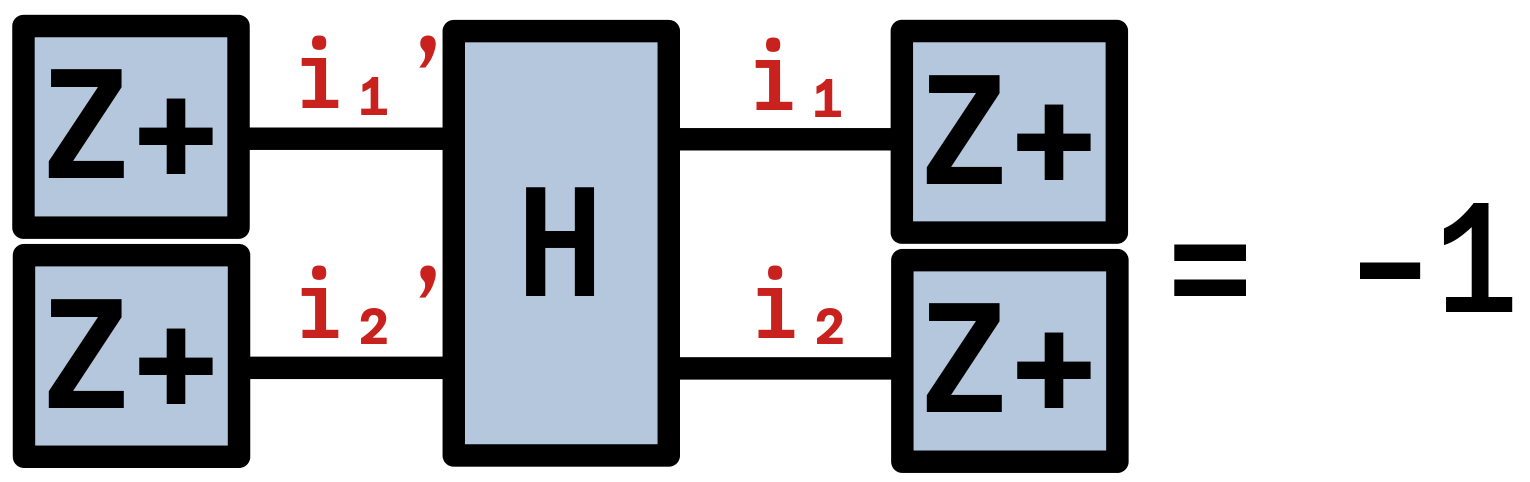
\includegraphics[width=0.2\textwidth]{
  slides/assets/Zp1Zp2HZp1Zp2.png
}
\end{center}
\vspace*{0.0cm}
\end{onlyenv}

\begin{onlyenv}<3-3>
~\\
$\approx$ [-√2, -1, 1, √2]
\end{onlyenv}

\begin{onlyenv}<4->
\vspace*{0.0cm}
\begin{center}
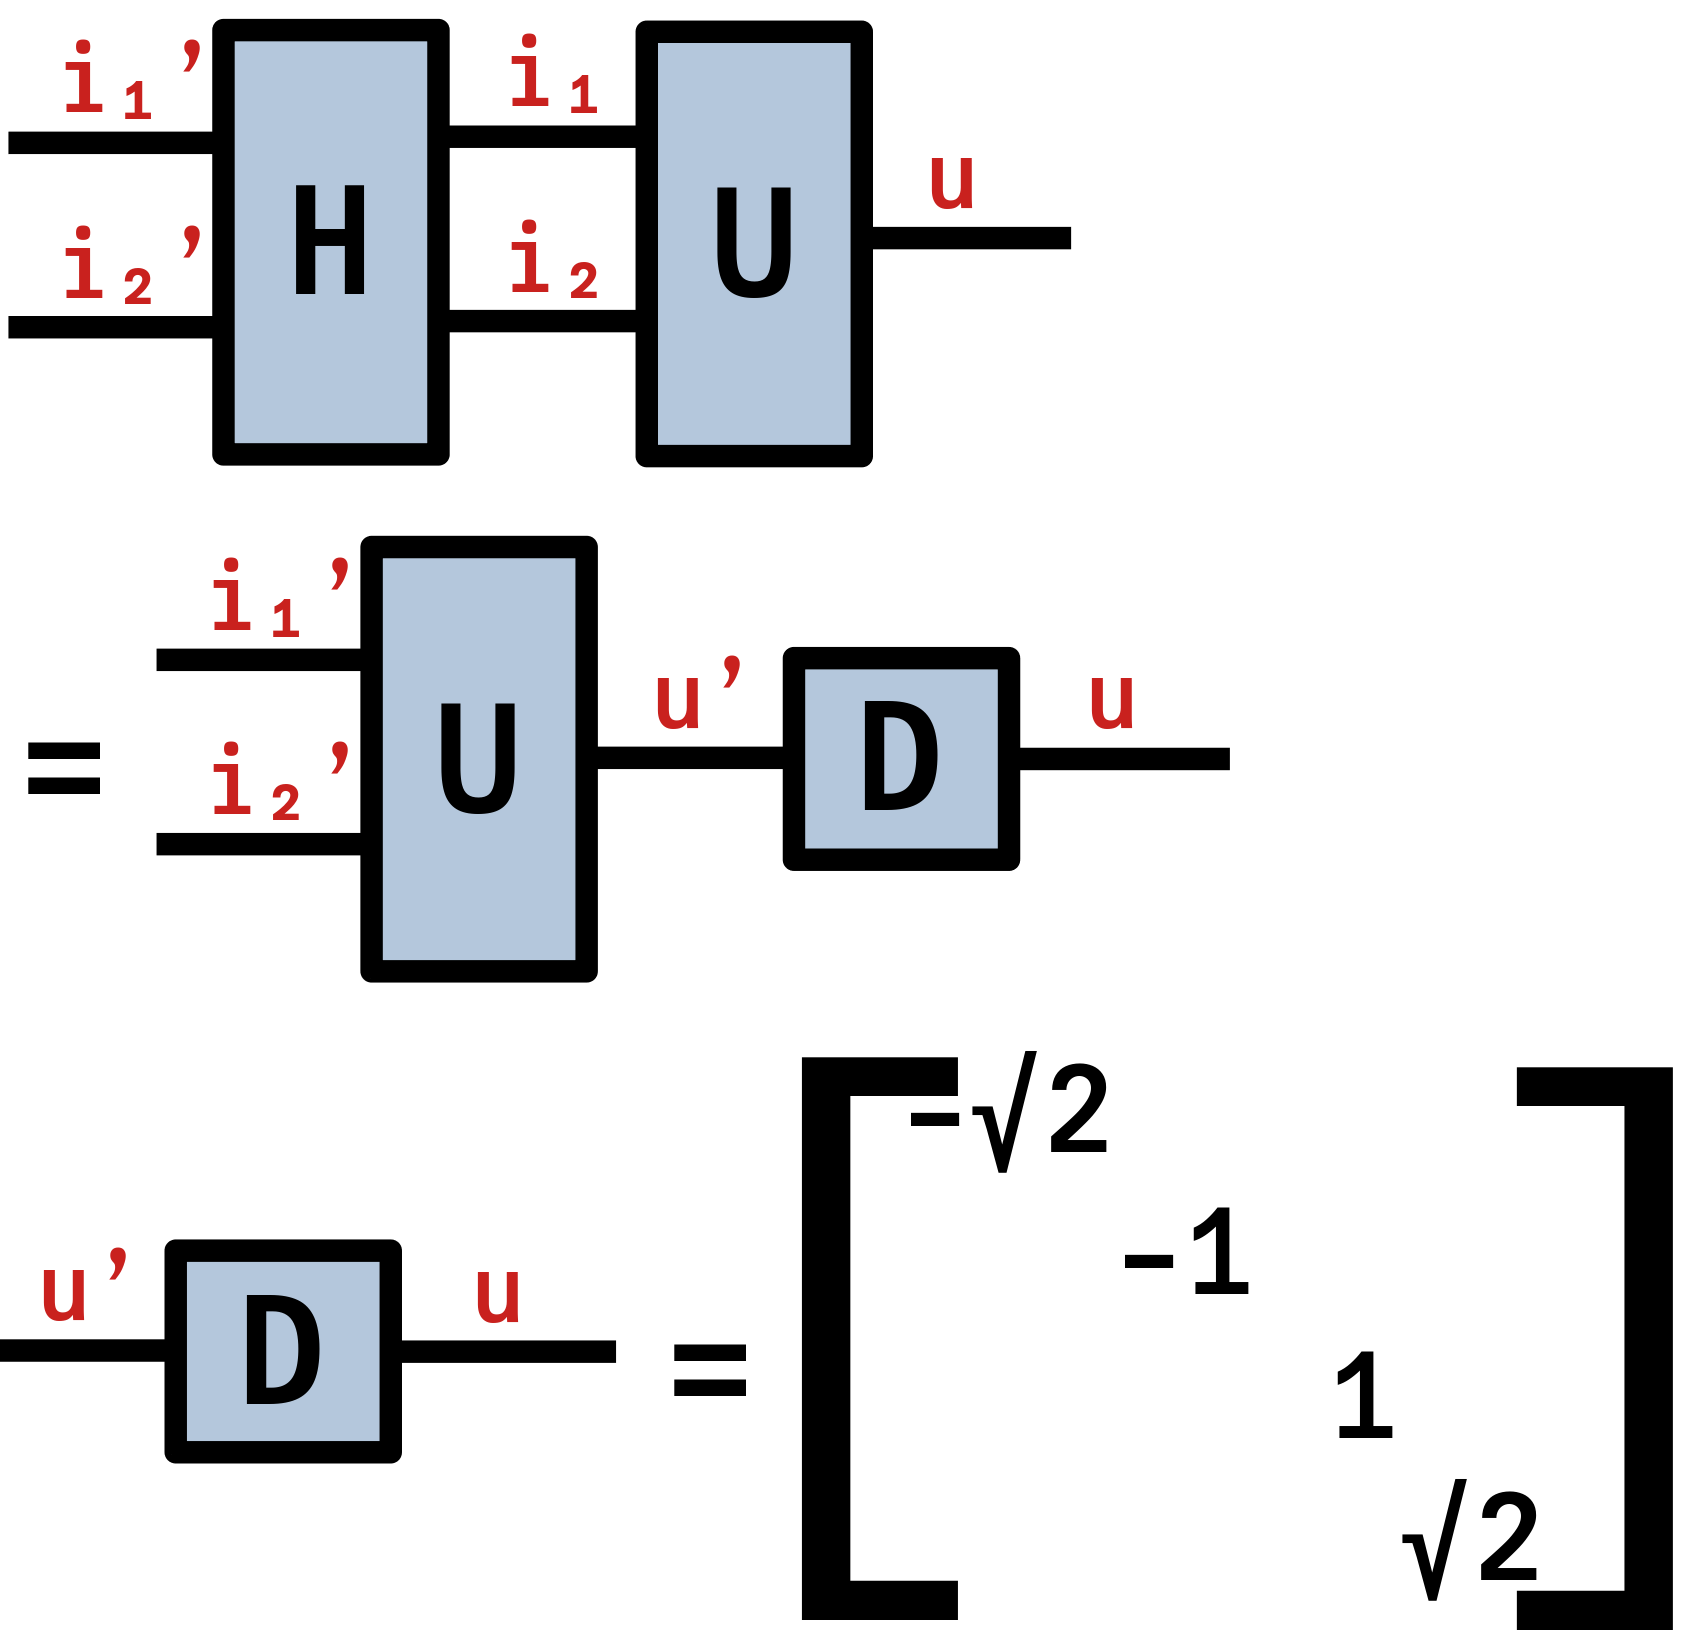
\includegraphics[width=0.2\textwidth]{
  slides/assets/eigen_H.png
}
\end{center}
\vspace*{0.0cm}
\end{onlyenv}

\end{column}

\end{columns}

\end{frame}
